\documentclass{article}
% translate with >> pdflatex -shell-escape <file>

% This file is used as unit test for pgfplots, copyright by Christian Feuersaenger.
% 
% See
%   http://pgfplots.sourceforge.net/pgfplots.pdf
% for pgfplots.
%
% Any required input files (for <plot table> or <plot file> or the table package) can be downloaded
% at
% http://www.ctan.org/tex-archive/graphics/pgf/contrib/pgfplots/doc/latex/
% and
% http://www.ctan.org/tex-archive/graphics/pgf/contrib/pgfplots/doc/latex/plotdata/

\usepackage{pgfplots}
\pgfplotsset{compat=newest}

\pagestyle{empty}

\begin{document}

\pgfplotsset{
	error bars/.cd,
	y dir=both,
	y explicit,
	x dir=both,
	x explicit,
	error bar style={black,dotted,error bars/error mark=square*,error bars/error mark options={current plot style}},
}


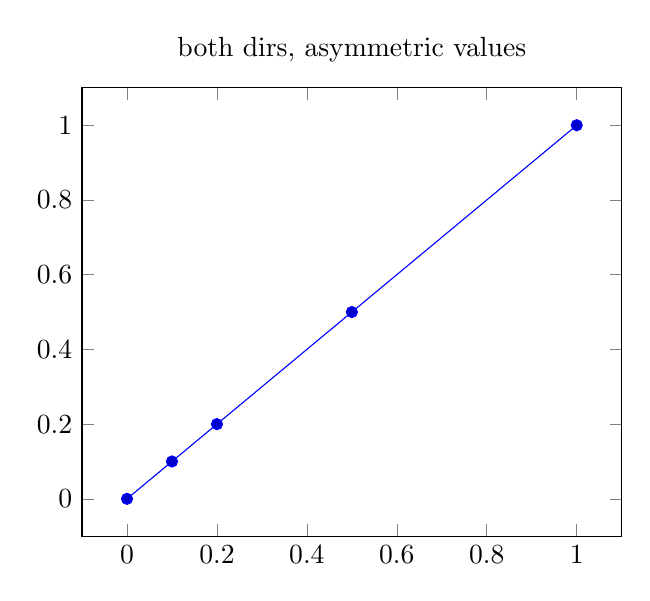
\begin{tikzpicture}
\begin{axis}[title={both dirs, asymmetric values},]
\addplot+[
]
	table[
		x error plus=ex+,
		x error minus=ex-,
		y error plus=ey+,
		y error minus=ey-,
	] {
	x y ex+ ey+ ex- ey-
	 0 0    0.5 0.1   0.1 0.05
	 0.1 0.1     0.05 0.2  0 0
	 0.2 0.2  	  0 0.05  1 0.2
	 0.5 0.5    0.1 0.2 0.2 0.1
	 1 1    0.3 0.1 0.3 0.1
	};
\end{axis}
\end{tikzpicture}
\end{document}
